\chapter{初等数论 Elementary Number Theory}

\section{Farey级数, Pell方程与连分数}

\subsection{Farey级数}

\begin{definition}{Farey级数}
	设正整数$n$, 将所有分母不超过$n$的最简分数按分数值递增排列, 称所得到的序列为\textit{$n$阶Farey级数}. 
\end{definition}

\begin{proposition}{}
	若$a/b, a'/b'$是$n$阶Farey级数中相邻两项, 则$b+b' \geq n+1$, $ba'-ab'=\pm 1$. 
\end{proposition}
\begin{proof}
	\underline{\textbf{证法一}}~~不妨设$a'/b' > a/b$. 我们可以找到整数$x,y$使得$bx-ay=1$且$n-b < y \leq n$, 因为$ay \equiv -1 \mod b$在$n-b+1 \sim n$中至少存在一个解$y$. 下面证明$a'/b'=x/y$, 从而$y=b',x=a'$: 
	
	用反证法. 注意到$\frac{x}{y} = \frac{a}{b} + \frac{1}{by} > \frac{a}{b}$, 从而$\frac{x}{y} > \frac{a'}{b'}$. 但是$$\frac{x}{y} - \frac{a'}{b'} = \frac{b'x-a'y}{b'y} \geq \frac{1}{b'y},\qquad \frac{a'}{b'} - \frac{a}{b} = \frac{a'b-ab'}{bb'} \geq \frac{1}{bb'}, $$
	可得$\frac{1}{by} = \frac{x}{y} - \frac{a}{b} \geq \frac{1}{b'y}+\frac{1}{bb'}$, 从而$b' \geq y+b >n$, 矛盾. 
	
	\underline{\textbf{证法二}}~~可以认为Farey级数的排序方式就是用一根扫描棒从$y$轴负方向出发, 沿逆时针方向依次扫过第四,一象限, 途中每碰到一个点就记录其坐标$A_i=(x_i,y_i)$. 不难发现若$A_i$与$A_{i+1}$相邻, 那么$\Delta A_iOA_{i+1}$中恰有$3$个边点且无内点, 所以$[A_iOA_{i+1}] = \frac{1}{2}$. 另一方面, 我们知道$$[A_iOA_{i+1}] = \frac{|x_{i+1}y_i-x_iy_{i+1}|}{2} = \frac{1}{2}.$$
	所以结论(2)成立. 
\end{proof}

\begin{corollary}{}
	给定实数$x$与正整数$n$, 存在互素整数$a,b$满足$0<b \leq n$且$$\big| x-\frac{a}{b} \big| \leq \frac{1}{b(n+1)}.$$
\end{corollary}
\begin{proof}
	用$n$阶Farey级数来逼近. 设$f_1<\cdots < f_d$是$n$阶Farey级数在$[x-\delta ,x+\delta]$中的项, $f_i=\frac{a_i}{b_i}$. 希望将$[x-\delta ,x+\delta]$分划为$[f_1,g_1]\cup [g_1,f_2] \cup \cdots \cup [g_{d-1},f_d]$且$g_i-f_i \leq \frac{1}{(n+1)b_i}, f_{i+1}-g_i \leq \frac{1}{(n+1)b_{i+1}}$, 从而对于$x \in [f_i,g_i]$或$[g_{i-1},f_i]$, 取$f_i$即得到所求逼近分数. 只需令$$\frac{a_i}{b_i} + \frac{1}{(b_i+b_{i+1})b_i}\geq g_i \geq \frac{a_{i+1}}{b_{i+1}} - \frac{1}{(b_i+b_{i+1})b_{i+1}}. $$
	取$g_i=\frac{a_i+a_{i+1}}{b_i+b_{i+1}}$即可. 
\end{proof}

\begin{corollary}{}
	给定无理数$x$, 存在无穷多对互素整数$(p,q)$使得$$\big| x - \frac{p}{q} \big| < \frac{1}{q^2}.$$
\end{corollary}
\begin{proof}
	由上方的推论, 对正整数$n$, 存在$(p_n,q_n)$使得$|x-\frac{p_n}{q_n}| < \frac{1}{q_n(n+1)} < \frac{1}{q_n^2}$. 假设$\{ q_n \}$有界, 那么$\{ q_n \},\{ p_n \}$均有界, 从而存在$n$使得对无穷多个$i$都有$|q_nx-p_n| = |q_ix-p_i| < \frac{1}{i+1}$. 令$i \to \infty$可得$x=\frac{p_n}{q_n}$, 与$x$是无理数矛盾. 
\end{proof}

注意, 若$x$是有理数, 则只存在有限对互素整数$(p,q)$满足上述条件. 否则考虑满足该条件的数列$\{ p_n \},\{ q_n \}$并记$x=a/b$. 对于某些$n$(待定)我们有$|q_na-p_nb|<\frac{|b|}{|q_n|}$, 注意到若右侧有上界$1$那么存在不同的$n,m$使得$\frac{p_n}{q_n}=\frac{p_m}{q_m}=\frac{a}{b}$, 矛盾. 这一点是易于证明的, 因为我们有$\{ q_n \}$无界(否则$\{ p_n \},\{ q_n \}$均有界). 


\begin{theorem}{处理方程$x^2+y^2=n$}
	将$(x,y)$映射到$yx^{-1} \mod n$的映射是$\{ (x,y) \in \mathbb{N}_1^2:\gcd (x,y)=1, x^2+y^2=n \}$到$\{ z \in \mathbb{Z}/n : z^2 \equiv -1 \mod n \}$的双射. 
\end{theorem}
\begin{proof}
	(1) 证明映射是良定义的, 也就是说对于$z \equiv yx^{-1}  \mod n$, 有$z^2 \equiv -1 \mod n$. 实际上$0 \equiv x^2+y^2 \equiv x^2(z^2+1) \mod n$, 又$x,n$互素, 故$z^2 \equiv -1 \mod n$. 
	
	(2) 证明该映射是单射. 假设存在不同的$(x_1,y_1),(x_2,y_2)$使得其对应的$z$相同, 即有$x_1y_2 \equiv x_2y_1 \mod n$. 实际上可以估计出$|x_1y_2-x_2y_1|<n$, 因为$$n^2 = (x_1^2+y_1^2)(x_2^2+y_2^2) = (x_1y_2-x_2y_1)^2 + (x_1y_1+x_2y_2)^2.$$
	从而, $x_1y_2=x_2y_1$, 那么$x_1 = x_2$, 矛盾.
	
	(3) 
	
	\begin{center}
		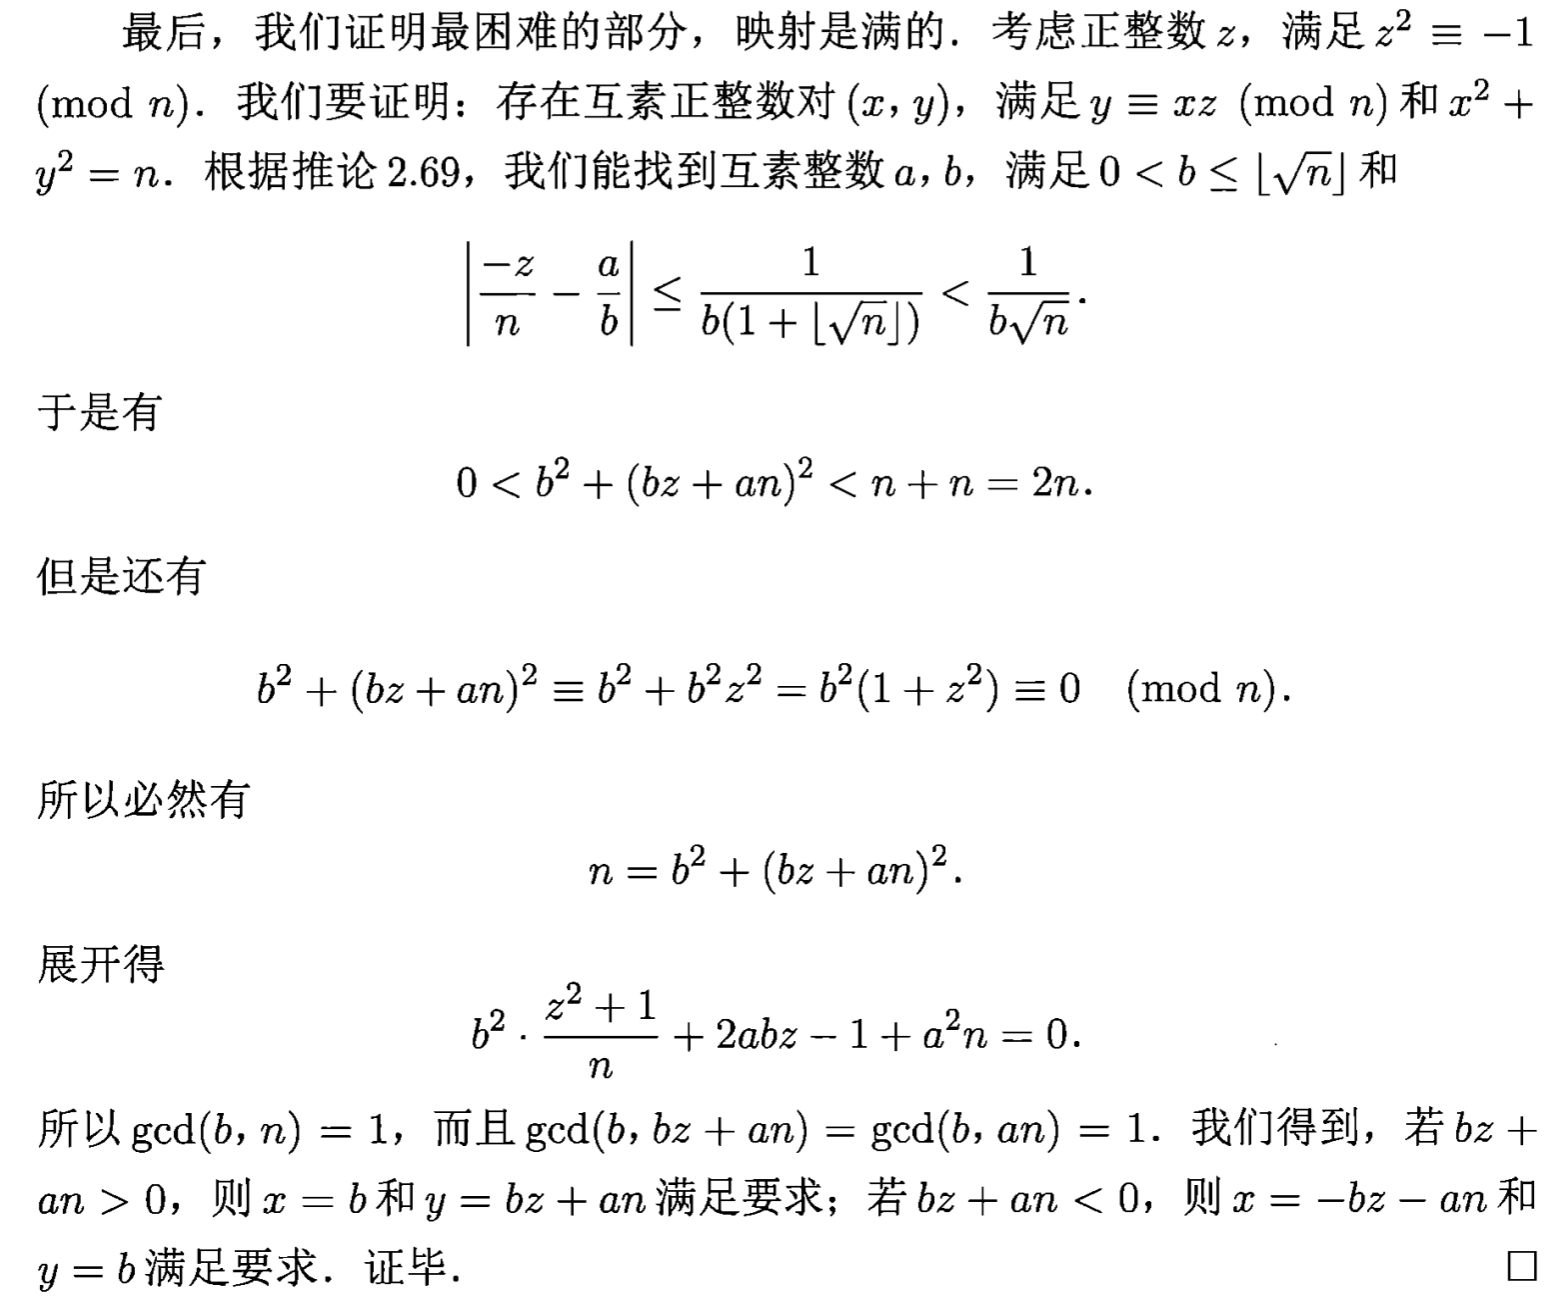
\includegraphics[width=13cm]{attachment/iShot_2024-01-06_21.42.59.png}
	\end{center}
	 
\end{proof}

\begin{theorem}{处理方程$x^2-dy^2=1$}
	设$d$是非平方正整数, 则方程$x^2-dy^2=1$存在正整数解. 
\end{theorem}
\begin{proof}
	给定$d$使得$\sqrt{d}$是无理数, 那么存在无穷多对$(x,y)$使得$|x-y\sqrt{d} |<\frac{1}{y}$, 特别地$$|x^2-dy^2| < \frac{1}{y}(x+y\sqrt{d}) < \frac{1}{y}(2y\sqrt{d} + \frac{1}{y}) < 3\sqrt{d}.$$
	所以存在(非零)整数$k$使得$x^2-dy^2=k$有无穷多对解. 
	
	\begin{center}
		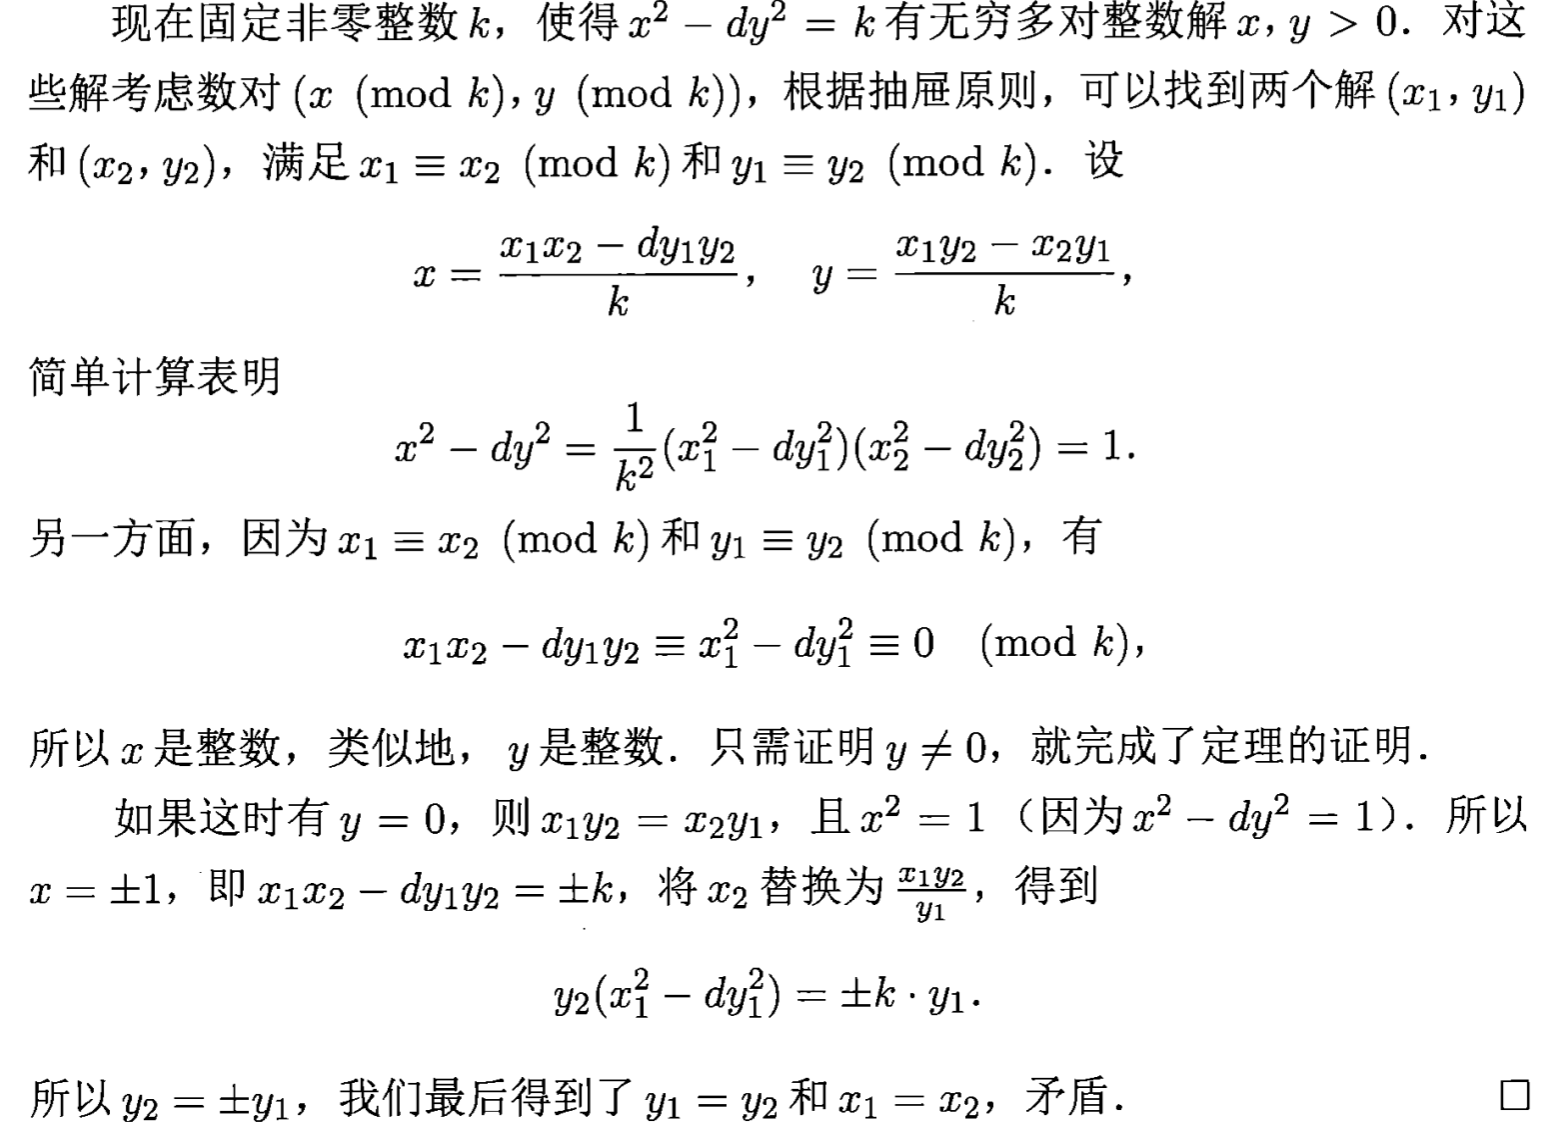
\includegraphics[width=13cm]{attachment/iShot_2024-01-06_21.53.15.png}
	\end{center}
\end{proof}

\subsection{连分数}

给定自然数序列$\{ q_n \}$, 定义序列$\{ R_n \}$: $$R_0=q_0, R_1=q_0+\frac{1}{q_1}, \cdots ,R_n = q_0 + \dfrac{1}{q_1 
          + \dfrac{1}{q_2 
          + \cdots \dfrac{1}{q_{n-1}+\dfrac{1}{q_n}}  } }.$$
我们也将$R_n$记作$[q_0;q_1,\cdots ,q_n]$. 


a) 对每个有理数$\frac{m}{l}$, 均存在唯一的$n$和$\{ q_n \}$使得$q_n \neq 1$且$R_n=\frac{m}{l}$. (提示: 利用Euclid算法)

b) 渐进分数序列$\{ R_n \}$满足以下不等式: $$\exists m,l,~ R_0<R_2< \cdots <R_{2k} < \frac{m}{l} < R_{2k+1} < R_{2k-1} < \cdots < R_1.$$

c) 每个无穷连分数(定义为数列$\{ R_n \}$的极限)都存在, 且为无理数. 

d) 可以按照如下方式递归地构造$R_k$的分子$P_k$与分母$Q_k$. 
$$P_0=q_0, P_1=q_0q_1+1, P_k=P_{k-1}q_k+P_{k-2}~(k \geq 2); $$
$$Q_0=1, Q_1=q_1, Q_k=Q_{k-1}q_k+Q_{k-2}~(k \geq 2).$$

e) 相邻两项渐进分数的差: $$\frac{P_{k+1}}{Q_{k+1}} - \frac{P_k}{Q_k} = \frac{(-1)^k}{Q_{k+1}Q_k}}. $$
\begin{proof}
	问题的关键是计算$P_{k+1}Q_k-Q_{k+1}P_k$. 实际上, $$P_{k+1}Q_k-Q_{k+1}P_k = (P_kq_{k+1}+P_{k-1})Q_k-(Q_kq_{k+1}+Q_{k-1})P_k = -(P_kQ_{k-1}-Q_kP_{k-1}) = \cdots = (-1)^k. $$
\end{proof}

f) 估计渐进分数的误差: 对于实数$x$和渐进分数序列$\{ \frac{P_n}{Q_n} \}$, $$\big| x-\frac{P_k}{Q_k} \big| \leq \frac{1}{Q_kQ_{k+1}} \leq \frac{1}{Q_k^2}. $$


\subsection{Pell方程}

\begin{theorem}{第一类Pell方程}
	设$(x_1,y_1)$是方程$x^2-dy^2=1$(其中$\sqrt{d}$是无理数)的最小解, 则一般解$(x_n,y_n)$有如下表达形式: 
	
	\begin{itemize}
		\item $x_n+y_n\sqrt{d} = (x_1+y_1\sqrt{d})^n$; 
		\item $x_{n+1}=x_1x_n+dy_1y_n,\qquad y_{n+1}=y_1x_n+x_1y_n$; 
		\item $x_{n+2}=(2x_1) x_{n+1}-x_n,\qquad y_{n+2} = (2x_1)y_{n+1}-y_n$; 
		\item $x_n = \frac{1}{2}\ssb{(x_1+y_1\sqrt{d})^n + (x_1-y_1\sqrt{d})^n},\qquad y_n = \frac{1}{2\sqrt{d}}\ssb{(x_1+y_1\sqrt{d})^n - (x_1-y_1\sqrt{d})^n}$; 
		\item 设$\sqrt{d}$的循环连分数周期为$\ell$, 渐进分数为$\{ \frac{P_n}{Q_n} \}$. 则$$(x_n,y_n) = \begin{cases}
 (P_{n\ell-1},Q_{n\ell -1}), & \text{ if } 2 \mid \ell \\
 (P_{2n\ell-1},Q_{2n\ell -1}).  & \text{ if } 2 \nmid \ell
\end{cases}$$
	\end{itemize}
\end{theorem}
\begin{proof}
	(1) 先证明第一种表示形式. 
	
	首先, 容易验证若$x_n+y_n\sqrt{d} = (x_1+y_1\sqrt{d})^n$, 由二项式定理我们有$x_n-y_n\sqrt{d} = (x_1-y_1\sqrt{d})^n$, 从而$$x_n^2-dy_n^2 = (x_1^2-dy_1^2)^n = 1.$$
	
	接着, 考虑方程的正整数解$(x,y)$. 记$z_1 = x_1+y_1 \sqrt{d}$, $z = x+y\sqrt{d}$. 由于$z \geq z_1$, 存在正整数$n$使得$z_1^n \leq z < z_1^{n+1}$. 计算$$\frac{z}{z_1^n} = (x+y\sqrt{d})(x_1-y_1\sqrt{d})^n =: u+v\sqrt{d},\qquad (x-y\sqrt{d})(x_1+y_1\sqrt{d})^n = u-v\sqrt{d}. $$
	注意到$u^2-dv^2 = (x^2-dy^2)(x_1^2-dy_1^2)^n = 1$. 现在$1 \leq u+v\sqrt{d} < z_1$, 假设$u+v\sqrt{d} > 1 > u-v\sqrt{d} >0$, 显然$u>0,v>0$. 从而我们得到了比$(x_1,y_1)$更小的解$(u,v)$, 矛盾. 因此$z = z_1^n$. 
	
	(2) 从(1)的证明中自然有第二条和第四条, 由第四条又可以得到第三条(利用线性递推公式)和第五条(此处略). 
\end{proof}
\vspace{1em}

\noindent
\textbf{\color{example} 例2.77.}~是否存在整数$a,b>1$, 使得$ab+1$和$ab^3+1$都是平方数? 
\vspace{1em}

接下来处理$ax^2-by^2=1$, 其中$a,b$为正整数. 特别地, 当$ab>1$是平方数时方程无正整数解. 
\vspace{1em}

\noindent
\textbf{\color{example} 例2.79.}~证明: 不存在正整数$a,b$使得$2a^2+1,2b^2+1,2(ab)^2+1$都是平方数. 

\begin{theorem}{}
	设正整数$a,b$满足$ab>1$不是平方数. 设$(x_1,y_1)$是方程$ax^2-by^2=1$的最小正整数解, $(u_n,v_n)$是方程$u^2-abv^2=1$的一般正整数解. 设方程$ax^2-by^2=1$的一般正整数解为$(x_n,y_n)$, 则: 
	
	\begin{itemize}
		\item $x_n=x_1u_n+by_1v_n,\qquad y_n=y_1u_n+ax_1x_n$; 
		\item $x_{n+2} = 2u_1x_{n+1}-x_n,\qquad y_{n+2} = 2u_1y_{n+1}-y_n$. 
	\end{itemize}
\end{theorem}

\begin{proposition}{两类Pell方程最小解的联系}
	设正整数$d$不是平方数, 使得方程$x^2-dy^2=-1$有正整数解. 设$(x_0,y_0)$是最小的正整数解, 则$(x_1,y_1)$满足$x_1+y_1\sqrt{d} = (x_0+y_0\sqrt{d})^2$是方程$x^2-dy^2=1$的最小正整数解. 
\end{proposition}
\begin{proof}
	记$(x_2,y_2)$是$x^2-dy^2=1$的最小整数解, $z_i=x_i+y_i\sqrt{d}$. 由上方定理可知, 存在正整数$n$使得$z_1=z_0^2=z_2^n$, 我们需要$n=1$, 即$n \geq 2$会得到$z_2^n \geq z_2^2 > z_0^2$矛盾, 于是只需证明$z_2>z_0$. 若不然, 计算$$\frac{z_0}{z_2} = (x_0+y_0\sqrt{d})(x_2-y_2\sqrt{d})=:u+v\sqrt{d} \quad \Rightarrow \quad u^2-dv^2=(x_0^2-dy_0^2)(x_2^2-dy_2^2)=-1. $$
	注意此时$z_0>u+v\sqrt{d}>1$, $0>u-v\sqrt{d}>-1$, 容易说明$u,v>0$, 从而得到矛盾. 
\end{proof}
\vspace{1em}

\noindent
\textbf{\color{example} 例2.82.}~求所有的正整数$m,n$, 使得$3^m = 2n^2+1$. 
\vspace{1em}

\noindent
\textbf{\color{example} 例2.83.}~证明: 存在无穷多个正整数$n$, 使得$n^2+1$有两个相差为$n$的正因子. 
\vspace{1em}

\noindent
\textbf{\color{example} 例2.84.}~证明: 存在无穷多对正整数组$(a,b,c)$构成等差数列且$ab+1,bc+1,ca+1$均为平方数. 


\vspace{2em}

由$\sum_{n & = 1}^{\infty}a_n$收敛, 可知任取$\varepsilon >0$, 存在$N>0$使得所有$n>N$和任意$p\geq 0$有$$(p+1)a_{n+p} \leq |a_n+\cdots +a_{n+p}| < \varepsilon .$$
固定$n$, 可知$\lim_{p\to \infty} (n+p)a_{n+p} = (n-1)\lim_{p\to \infty} a_{n+p} = 0$. 














